\documentclass[11pt]{article}
\usepackage[utf8]{inputenc}
\usepackage[T1]{fontenc}
\usepackage[brazilian]{babel}
\usepackage{graphicx}
\usepackage{longtable}
\usepackage{wrapfig}
\usepackage{rotating}
\usepackage[normalem]{ulem}
\usepackage{amsmath}
\usepackage{amsfonts}
\usepackage{amssymb}
\usepackage{amsthm}
\usepackage{capt-of}
\usepackage{hyperref}
\usepackage{geometry}
\usepackage{booktabs}
\usepackage{url}
\usepackage{hyperref}
\usepackage{multicol}
\usepackage{algorithm}
\usepackage{algorithmicx}
\usepackage[noend]{algpseudocode}
\usepackage[title]{appendix}
\usepackage{float}
\usepackage{xspace}
\usepackage{subcaption}

\theoremstyle{definition}
\newtheorem{defn}{Definição}
\newtheorem{fact}{Fato}

\newcommand{\Set}[1]{\left\{#1\right\}}
\newcommand{\Sum}[4]{\displaystyle\sum\limits_{#1 = #2}^{#3} #4}
\newcommand{\function}[3]{#1: #2 \rightarrow #3}
\newcommand{\transpose}[1]{#1^{T}}

\newcommand{\B}{\mathbb{B}}
\newcommand{\Bn}{\mathbb{B}^n}
\newcommand{\R}{\mathbb{R}}
\newcommand{\Rn}{\mathbb{R}^n}
\newcommand{\Z}{\mathbb{Z}}
\newcommand{\Zn}{\mathbb{Z}^n}

\newcommand{\argmax}[2]{\mathop{\mathrm{arg\,max}}\limits_{#1}\Set{#2}}

\newcommand{\qbf}{QBF\xspace}
\newcommand{\maxqbf}{MAX-QBF\xspace}
\newcommand{\maxkqbf}{MAX-KQBF\xspace}
\newcommand{\maxkqbffull}{\textit{MAX-QBF com mochila}\xspace}

\newcommand{\w}{w}
\newcommand{\W}{W}

\newcommand{\aij}{a_{i,j}}
\newcommand{\A}{A}

\newcommand{\grasp}{\textit{GRASP}\xspace}
\newcommand{\graspfull}{\textit{Greedy Randomized Adaptive Search Procedure}\xspace}
\newcommand{\bestImproving}{\textit{Best Improving}}
\newcommand{\firstImproving}{\textit{First Improving}}
\newcommand{\graspBest}{\textit{\grasp Best}\xspace}
\newcommand{\graspFirst}{\textit{\grasp First}\xspace}

\newcommand{\tabu}{\textit{Tabu}\xspace}
\newcommand{\tabufull}{\textit{Tabu Search}\xspace}
\newcommand{\tenureRatio}{\textit{Tenure Ration}\xspace}
\newcommand{\tabuVanilla}{\textit{\tabu Vanilla}\xspace}
\newcommand{\tabuMod}{\textit{\tabu com Intensificação e Diversificação}\xspace}

\newcommand{\genetic}{\textit{GA}\xspace}
\newcommand{\geneticfull}{\textit{\genetic Algorithm}\xspace}
\newcommand{\geneticVanilla}{\textit{\genetic Vanilla}\xspace}
\newcommand{\geneticSteady}{\textit{\genetic Steady}\xspace}

\newcommand{\tttfull}{Time-To-Target Plot\xspace}
\newcommand{\ttt}{TTT Plot\xspace}
\newcommand{\tttvaren}{\textit{Time-To-Target Solution Value}\xspace}
\newcommand{\tttvar}{\textit{Tempo para atingir valor alvo da solução}\xspace}
\newcommand{\qq}{\textit{Q-Q plot}\xspace}

\newcommand{\perfprof}{\textit{Performance Profile}}

\newcommand{\appendixref}[1]{Apêndice \ref{#1}}
\newcommand{\tref}[1]{Tabela \ref{#1}}
\newcommand{\fref}[1]{Figura \ref{#1}}
\newcommand{\aref}[1]{Algoritmo \ref{#1}}
\newcommand{\sref}[1]{Seção \ref{#1}}
\newcommand{\ssref}[1]{Subseção \ref{#1}}
\newcommand{\sssref}[1]{Subsubseção \ref{#1}}

\geometry{a4paper, left=20mm, top=35mm, bottom=35mm, right=20mm}

\author{Lucas Guesser Targino da Silva (203534)}
\date{\today}
\title{MO824 - Análise Comparativa entre as metaheurísticas \grasp, \tabu, e \genetic para a resolução do problema MAX-QBF com mochila}

\begin{document}

\maketitle

\section{Metaheurísticas}
\label{section:metaheuristics}

Nessa seção são descritas todas as metaheurísticas utilizadas ao longo do trabalho.

No desenvolvimento dos trabalhos anteriores, explorou-se variações de cada metaheurística, essas com diferentes parâmetros, estratégias construtivas, buscas locais, etc. Para cada metaheurística, foram selecionadas duas variações, as que apresentaram melhor desempenho, para serem utilizadas nas investigações deste trabalho.


\section{Metaheurísticas}
\label{section:metaheuristics}

Nessa seção são descritas todas as metaheurísticas utilizadas ao longo do trabalho.

No desenvolvimento dos trabalhos anteriores, explorou-se variações de cada metaheurística, essas com diferentes parâmetros, estratégias construtivas, buscas locais, etc. Para cada metaheurística, foram selecionadas duas variações, as que apresentaram melhor desempenho, para serem utilizadas nas investigações deste trabalho.

\begin{table}
    \centering
    \begin{tabular}{lllllllll}
        \toprule
        {} & instances & construction & alpha & local search    & iterations & best cost & weight & duration \\
        \midrule
        0  & 020       & default      & 0.2   & first improving & 1000       & 120       & 56     & 0.145    \\
        1  & 040       & default      & 0.2   & first improving & 1000       & 306       & 136    & 0.353    \\
        2  & 060       & default      & 0.2   & first improving & 1000       & 455       & 220    & 1.261    \\
        3  & 080       & default      & 0.2   & first improving & 1000       & 783       & 286    & 3.016    \\
        4  & 100       & default      & 0.2   & first improving & 1000       & 1213      & 335    & 6.056    \\
        5  & 200       & default      & 0.2   & first improving & 1000       & 3692      & 679    & 75.552   \\
        6  & 400       & default      & 0.2   & first improving & 1000       & 9756      & 1342   & 650.589  \\
        \bottomrule
    \end{tabular}
    \caption{grasp-first}
    \label{table:grasp-first}
\end{table}

\begin{table}
    \centering
    \begin{tabular}{lllllllll}
        \toprule
        {} & instances & construction & alpha & local search   & iterations & best cost & weight & duration \\
        \midrule
        0  & 020       & default      & 0.2   & best improving & 1000       & 120       & 56     & 0.074    \\
        1  & 040       & default      & 0.2   & best improving & 1000       & 295       & 137    & 1.765    \\
        2  & 060       & default      & 0.2   & best improving & 1000       & 491       & 212    & 1.981    \\
        3  & 080       & default      & 0.2   & best improving & 1000       & 795       & 284    & 4.242    \\
        4  & 100       & default      & 0.2   & best improving & 1000       & 1228      & 345    & 9.068    \\
        5  & 200       & default      & 0.2   & best improving & 1000       & 3766      & 677    & 100.731  \\
        6  & 400       & default      & 0.2   & best improving & 1000       & 10213     & 1343   & 973.293  \\
        \bottomrule
    \end{tabular}
    \caption{grasp-best}
    \label{table:grasp-best}
\end{table}

\subsection{\tabu}
\label{subsection:tabu}

A metaheurística \tabu é descrita no \aref{algorithm:tabu}.

Ambas as variações descritas nessa subseção usam:

\begin{enumerate}
    \item solução inicial a solução da estratégia construtiva do \grasp, \aref{algorithm:grasp-construction};
    \item busca local \bestImproving. Ela é similar a \bestImproving descrita na \ssref{subsection:grasp}, entretanto ela não considera a adição ou remoção de elementos que estão na lista tabu $T$ (a menos que eles levem a uma solução melhor do que $S^*$);
    \item \tenureRatio, parâmetro que controla o tamanho da lista tabu $T$, igual a $0.4$, o que significa que $T$ pode ter tamanho até 40\% do tamanho da entrada.
\end{enumerate}

A primeira variação, chamada \tabuVanilla, implementa \tabu com as características acima. A segunda variação, chamada \tabuMod, inclui estratégias de diversificação e intensificação, descritas nas \sssref{subsubsection:tabu-intensification} e \sssref{subsubsection:tabu-diversification}.

\subsubsection{Estratégia de Intensificação}
\label{subsubsection:tabu-intensification}

A estratégia de intensificação aumenta o tamanho da vizinhaça, ao invés de considerar 1 adição, 1 remoção e 1 troca, ela considera:

\begin{enumerate}
    \item 2 adições e 1 remoção;
    \item 2 remoções e 1 adição;
    \item 2 adições e 2 remoções;
\end{enumerate}

A intensificação é feita em torno da melhor solução conhecida. Ela é ativada quando passam-se muitas iterações (o critério de parada é definido como um número máximo de iterações, e ``muitas iterações'' significa 20\% número máximo de iterações) sem melhora na solução ótima e sem sua ativação.

\subsubsection{Estratégia de Diversificação}
\label{subsubsection:tabu-diversification}

A estratégia de diversificação constroi uma nova solução, utilizando a estratégia construtiva do GRASP, e recomeça a busca nesse outro local do espaço de solução. Além disso, antes de começar a busca, faz-se uma busca intensiva (usando a estratégia de intensificação) em torno dessa nova solução.

Seu critério de ativação é o mesmo da Estratégia de Intensificação, excetuando-se que Diversificação é ativada apenas quando Intensificação não é (no programa, há um registro separado para quando cada uma delas foi ativada pela última vez).

Assim, quando se passaram muitas iterações sem melhora na solução ótima, primeiro tenta-se intensificação. Caso essa falhe, executa-se a diversificação.

\subsubsection{\tabuVanilla}
\label{subsubsection:tabu-vanilla}

\begin{enumerate}
    \item Solução inicial: saída da estratégia construtiva do \grasp
    \item \tenureRatio: \textbf{0.4}
    \item Estratégia de busca local: \textbf{\bestImproving}
\end{enumerate}

\subsubsection{\tabuMod}
\label{subsubsection:tabu-mod}

\begin{enumerate}
    \item Solução inicial: saída da estratégia construtiva do \grasp
    \item \tenureRatio: \textbf{0.4}
    \item Estratégia de busca local: \textbf{\bestImproving}
    \item Adição das estratégias: \textbf{Intensificação e Diversificação}
\end{enumerate}

\subsection{\genetic}
\label{subsection:genetic}

A metaheurística \tabu é descrita no \aref{algorithm:genetic}.

Ambas as variações descritas nessa subseção usam:

\begin{enumerate}
    \item população inicial aleatória;
    \item tamanho da população igual a 100;
    \item seleção para reprodução em torneio: dois cromossomos são escolhidos aleatoriamente e o
    melhor dos dois (em relação à função de aptidão) é escolhido para continuar enquanto o outro é
    descartado.
    \item reprodução com \textit{two point crossover (2X)};
    \item Critério de parada: 1000 gerações;
\end{enumerate}

\subsubsection{\geneticVanilla}

A primeira variação, chamada \geneticVanilla, implementa \genetic conforme descrito na \ssref{subsection:genetic} com as seguintes adições/modificações:

\begin{enumerate}
    \item taxa de mutação igual a $0.5\%$;
    \item seleção da nova população: descendentes, substituindo-se o pior deles pelo melhor gene conhecido
\end{enumerate}

\subsubsection{\geneticSteady}

A segunda variação, chamada \geneticSteady, implementa \genetic conforme descrito na \ssref{subsection:genetic} com as seguintes adições/modificações:

\begin{enumerate}
    \item taxa de mutação igual a $1\%$;
    \item seleção da nova população: os 100 melhores genes entre mães e filhos (conhecida como \textit{Steady-State $\lambda + \mu$});
\end{enumerate}


\section{\tttfull (\ttt)}

\section{\perfprof}
\label{appendix:performance-profiles}

\begin{table}[H]
    \centering
        \begin{tabular}{|p{0.2\textwidth}||l|l|l|l|l|l|l|}

    \hline
    Problema & kqbf020 & kqbf040 & kqbf060 & kqbf080 & kqbf100 & kqbf200 & kqbf400 \\ \hline\hline
    \graspFirst & 0.145 & 0.353 & 1.261 & 3.016 & 6.056 & 75.552 & inf \\ \hline
    \graspBest & 0.074 & 1.765 & 1.981 & 4.242 & 9.068 & 100.731 & inf \\ \hline
    \tabuVanilla & 0.997 & 2.707 & 5.427 & 10.318 & 17.549 & 160.816 & inf \\ \hline
    \tabuMod & 0.255 & 1.218 & 5.662 & inf & 17.294 & 444.594 & inf \\ \hline
    \geneticVanilla & 0.974 & 3.200 & 5.529 & 9.627 & 15.386 & 62.351 & inf \\ \hline
    \geneticSteady & 3.015 & 10.860 & 23.954 & 46.665 & 76.459 & 254.404 & inf \\ \hline
    \end{tabular}
    \caption{Dados utilizados na confecção do \perfprof. \textit{inf} acima significa que o algoritmo não consegui resolver o problema, isto é, não encontrou uma solução com valor pelo menos o valor definido para o problema em questão.}
    \label{tab:data-perfprof}
\end{table}

\begin{figure}[H]
    \centering
    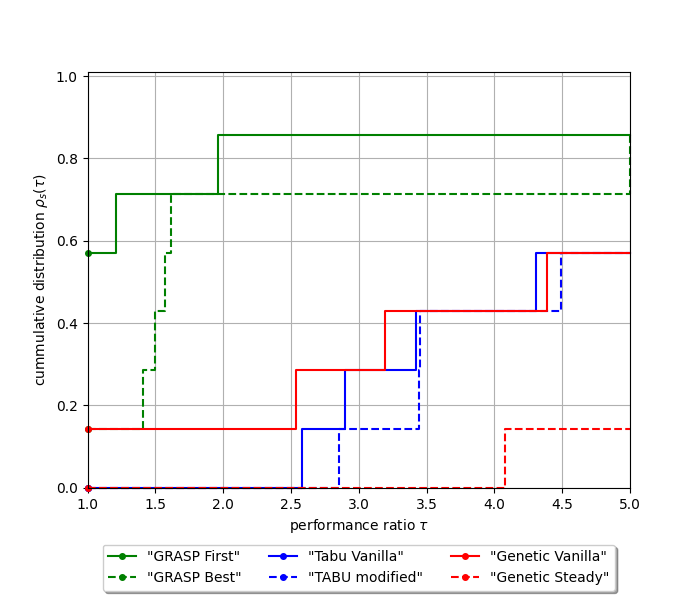
\includegraphics[width=\textwidth]{figure/performance_profile/performance_profile_thmax_5.0.png}
    \caption{Gráfico de \perfprof no intervalo $[1, 5]$}
    \label{fig:performance-profile-5}
\end{figure}

\begin{figure}[H]
    \centering
    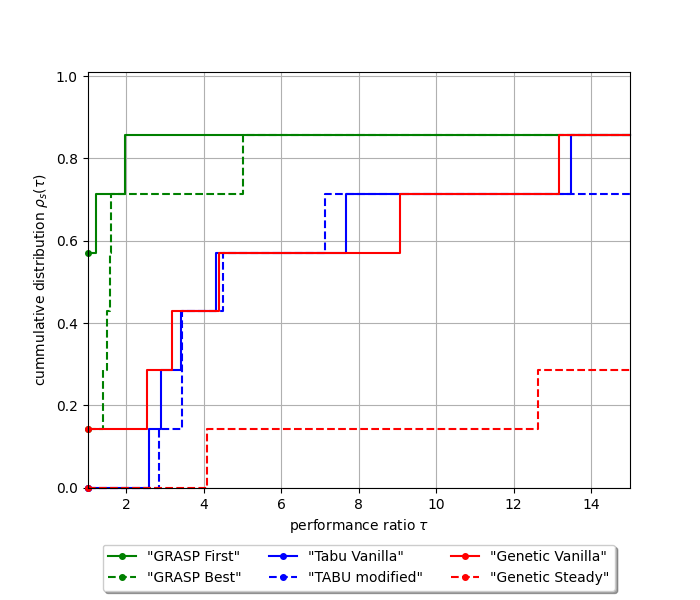
\includegraphics[width=\textwidth]{figure/performance_profile/performance_profile_thmax_15.0.png}
    \caption{Gráfico de \perfprof no intervalo $[1, 15]$}
    \label{fig:performance-profile-15}
\end{figure}

\begin{figure}[H]
    \centering
    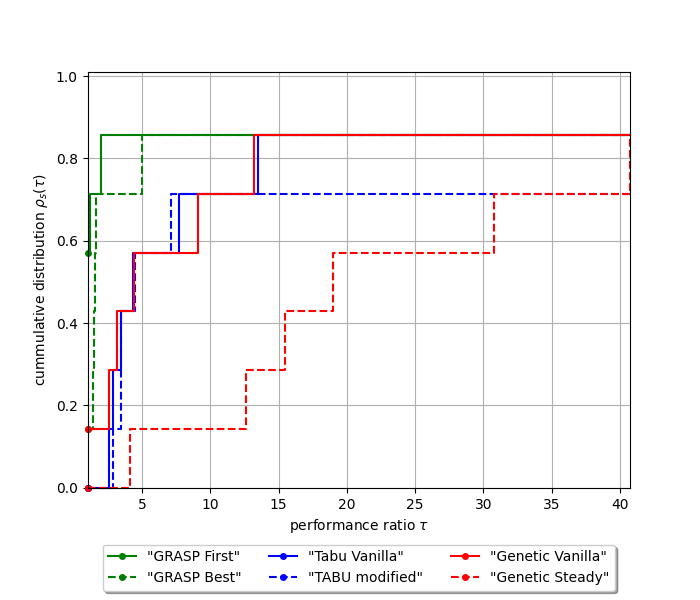
\includegraphics[width=\textwidth]{figure/performance_profile/performance_profile_thmax_None.png}
    \caption{Gráfico de \perfprof no intervalo $r_M$ (calculado automaticamente pelo software de plot).}
    \label{fig:performance-profile-max}
\end{figure}

\section{Melhores Soluções}
\label{section:best-solutions}

\textbf{Aviso}: Qualquer anlálise da tolerância aceita, em relação à melhor solução, dever levar a aplicação em consideração. Para esse trabalho, não há uma aplicação específica, de forma que é difícil apontar uma tolerância aceitável. mas considerando que estão sendo analisadas heurísticas, para fins de análise, qualquer tolerância dentro de 5\% será considerada aceitável.

\subsection{Resultados}
\label{subsection:best-solutions-results}
\begin{table}[H]
    \centering
    \begin{tabular}{|c|c|c|c|}
        \hline
        \textbf{Metaheurística} & \textbf{Instância} & \textbf{Melhor Solução} & \textbf{\% do Melhor} \\\hline\hline
        \geneticVanilla         & kqbf040            & 303                     &  1.62                   \\\hline
        \geneticSteady          & kqbf040            & 305                     &  0.97                   \\\hline
        \graspFirst             & kqbf040            & 306                     &  0.64                   \\\hline
        \graspBest              & kqbf040            & 295                     &  4.22                   \\\hline
        \tabuVanilla            & kqbf040            & 308                     &  0.00                   \\\hline
        \tabuMod                & kqbf040            & 303                     &  1.62                   \\\hline\hline
        \geneticVanilla         & kqbf060            & 481                     &  2.03                   \\\hline
        \geneticSteady          & kqbf060            & 453                     &  7.73                   \\\hline
        \graspFirst             & kqbf060            & 455                     &  7.33                   \\\hline
        \graspBest              & kqbf060            & 491                     &  0.00                   \\\hline
        \tabuVanilla            & kqbf060            & 491                     &  0.00                   \\\hline
        \tabuMod                & kqbf060            & 491                     &  0.00                   \\\hline\hline
        \geneticVanilla         & kqbf080            & 766                     &  3.64                   \\\hline
        \geneticSteady          & kqbf080            & 781                     &  1.76                   \\\hline
        \graspFirst             & kqbf080            & 783                     &  1.50                   \\\hline
        \graspBest              & kqbf080            & 795                     &  0.00                   \\\hline
        \tabuVanilla            & kqbf080            & 783                     &  1.50                   \\\hline
        \tabuMod                & kqbf080            & 702                     & 11.69                   \\\hline
    \end{tabular}
    \caption{Melhor solução encontrada por cada metaheurística, para cada instância analisada. \% do Melhor é calculada como $100 \cdot \left(1 - \dfrac{s}{s^*}\right)$, sendo $s$ a solução da metaheurística em questão e $s^*$ a melhor solução encontrada para aquela instância.}
    \label{tab:best-solutions}
\end{table}

\subsection{Análise}
\label{subsection:best-solutions-analysis}

A \tref{tab:best-solutions} contém resultados com as melhores soluções encontradas por cada metaheurística para as instâncias selecionadas.

Para a instância kqbf040, todas as metaheurísticas encontraram soluções dentro de 5\% da melhor.

Para a instância kqbf060, \graspBest, \tabuVanilla e \tabuMod encontraram a mesma solução, e \geneticVanilla está dentro dos 5\%. Já \geneticSteady e \graspBest não encontraram uma solução satisfatória.

Para a instância kqbf080, a única que teve desempenho não satisfatório foi \tabuMod.

Em geral, as melhores metaheurísticas foram \tabuVanilla, \graspBest, \geneticVanilla, nessa ordem. Elas forma as únicas a ficaram dentro da tolerância de 5\% nas três instâncias. \tabuVanilla e \graspBest obtiveram duas vezes a melhor solução, sendo que a segunda foi melhor na média.




\bibliographystyle{ieeetr}
\bibliography{bibliography}


\begin{appendices}

\section{\maxkqbffull (\maxkqbf)}
\label{appendix:max-kqbf}

\begin{defn}[Conjunto Binário]
    $\B = \Set{0, 1}$
\end{defn}

\begin{defn}[Função Binária Quadrática (\qbf)]
    É uma função $\function{f}{\Bn}{\Z}$ da forma:
    $$
        f(x)
        = \Sum{j}{1}{n}{x_i \cdot \aij \cdot x_j}
        = \transpose{x} \cdot \A \cdot x
    $$
    em que $\aij \in \Z, \ \forall i,j \in \Set{1, \cdots, n}$ e $\A$ é a matriz $n$ por $n$ induzida pelos $\aij$.
\end{defn}

\begin{defn}[Problema de Maximização de uma Função Binária Quadrática (\maxqbf)]
Dada uma \qbf $f$, um \maxqbf é um problema da forma:
$$
    \max\limits_{x} f(x)
$$
\end{defn}

\begin{fact}
\maxqbf é NP-difícil \cite{bib:qbf}
\end{fact}

\begin{defn}[Maximum knapsack quadractic binary function (\maxkqbf)]
Dada uma \qbf $f$, um vetor $\w \in \Zn$\footnote{O problema original foi definido com números reais. Decidimos aqui utilizar inteiros por dois motivos. Primeiro, todas as instâncias fornecidas possuem apenas valores inteiros para $\aij, \w, \W$. Garante-se que os valores são sempre inteiros pois $\Z$ é fechado nas operações envolvidas: adição e multiplicação. Segundo, simplifica a implementação e comparações (não é necessário fazer comparação de números em ponto flutuante).}, e um valor $\W \in \Z$, um \maxkqbf é um problema da forma:
\begin{eqnarray*}
    \max & f(x) \\
    \mbox{subjected to} & \transpose{\w} x \leq \W \\
    & x \in \Bn
\end{eqnarray*}
\end{defn}

\section{Instance Generation}

The instances are generated randomly \cite{bib:instances-CVRP}, \cite{bib:constrained-knapsack}, \cite{bib:grasp-and-tabu}. For that, first the graph is generated, and then the weight of each vertex is chosen. The knapsack capacity is selected so that, on average, X percent of the vertices fit in it. The following subsections analyze each of those aspects.

Consider the parameters:
\begin{enumerate}
    \item $n$: number of vertices;
    \item $K$: average number of branches;
    \item $L$: maximum number of leaf vertices;
    \item $H$: the maximum value of an entry of the weight of each vertex;
    \item $m$: fraction of the average number of elements that fit in the knapsack;
\end{enumerate}

\subsection{How to Generate the Precedences}

The process of generating the precedences is specified in \algref{algorith:find-trees}, which uses \algref{algorith:generate-precedences}. The \figref{fig:precedence-generation} has an example of such procedure. The following parameters are used to control the generation:

\begin{algorithm}
    \caption{Find-Trees}
    \label{algorith:find-trees}
    \begin{algorithmic}[1]
        \Require{
            $\vertices$: vertices in the 2D plane,
            $K$: average number of branches,
            $L$: maximum number of leaf vertices
        }
        \State{$k \gets $ random number from 1 to $K$}
        \State{$\tuple{R, \mathcal{V}} \gets $ find $k$ clusters in $V$}
            \Comment{$R$: a set of centers}\\
            \Comment{$\mathcal{V}$: a set with each element being the set vertices of each cluster}
        \State{$\mathcal{T} \gets \emptyset$}
        \For{each pair $r \in R $ and $V' \in \mathcal{V}$}
            \If{$\abs{V'} \leqslant L$}
                \State{$T \gets $ tree with $r$ as the root node and $V'$ as the leaves}
            \Else
                \State{$T \gets $ tree with $r$ as the root node of the subtree Find-Trees($V', K, L$)}
            \EndIf
            \State{$\mathcal{T} \gets \mathcal{T} \cup \Set{T}$}
        \EndFor
        \\\Return{$\mathcal{T}$}
    \end{algorithmic}
\end{algorithm}

\begin{algorithm}
    \caption{Generate-Precedences}
    \label{algorith:generate-precedences}
    \begin{algorithmic}[1]
        \Require{
            $n$: number of vertices,
            $K$: average number of branches,
            $L$: maximum number of leaf vertices
        }
        \State{$V \gets $ generate $n$ points in the 2D plane randomly}
        \State{$\mathcal{T} \gets $ Find-Trees($V, K, L$)}
        \\\Return{$\mathcal{T}$}
    \end{algorithmic}
\end{algorithm}

\begin{figure}[ht!]
    \centering
    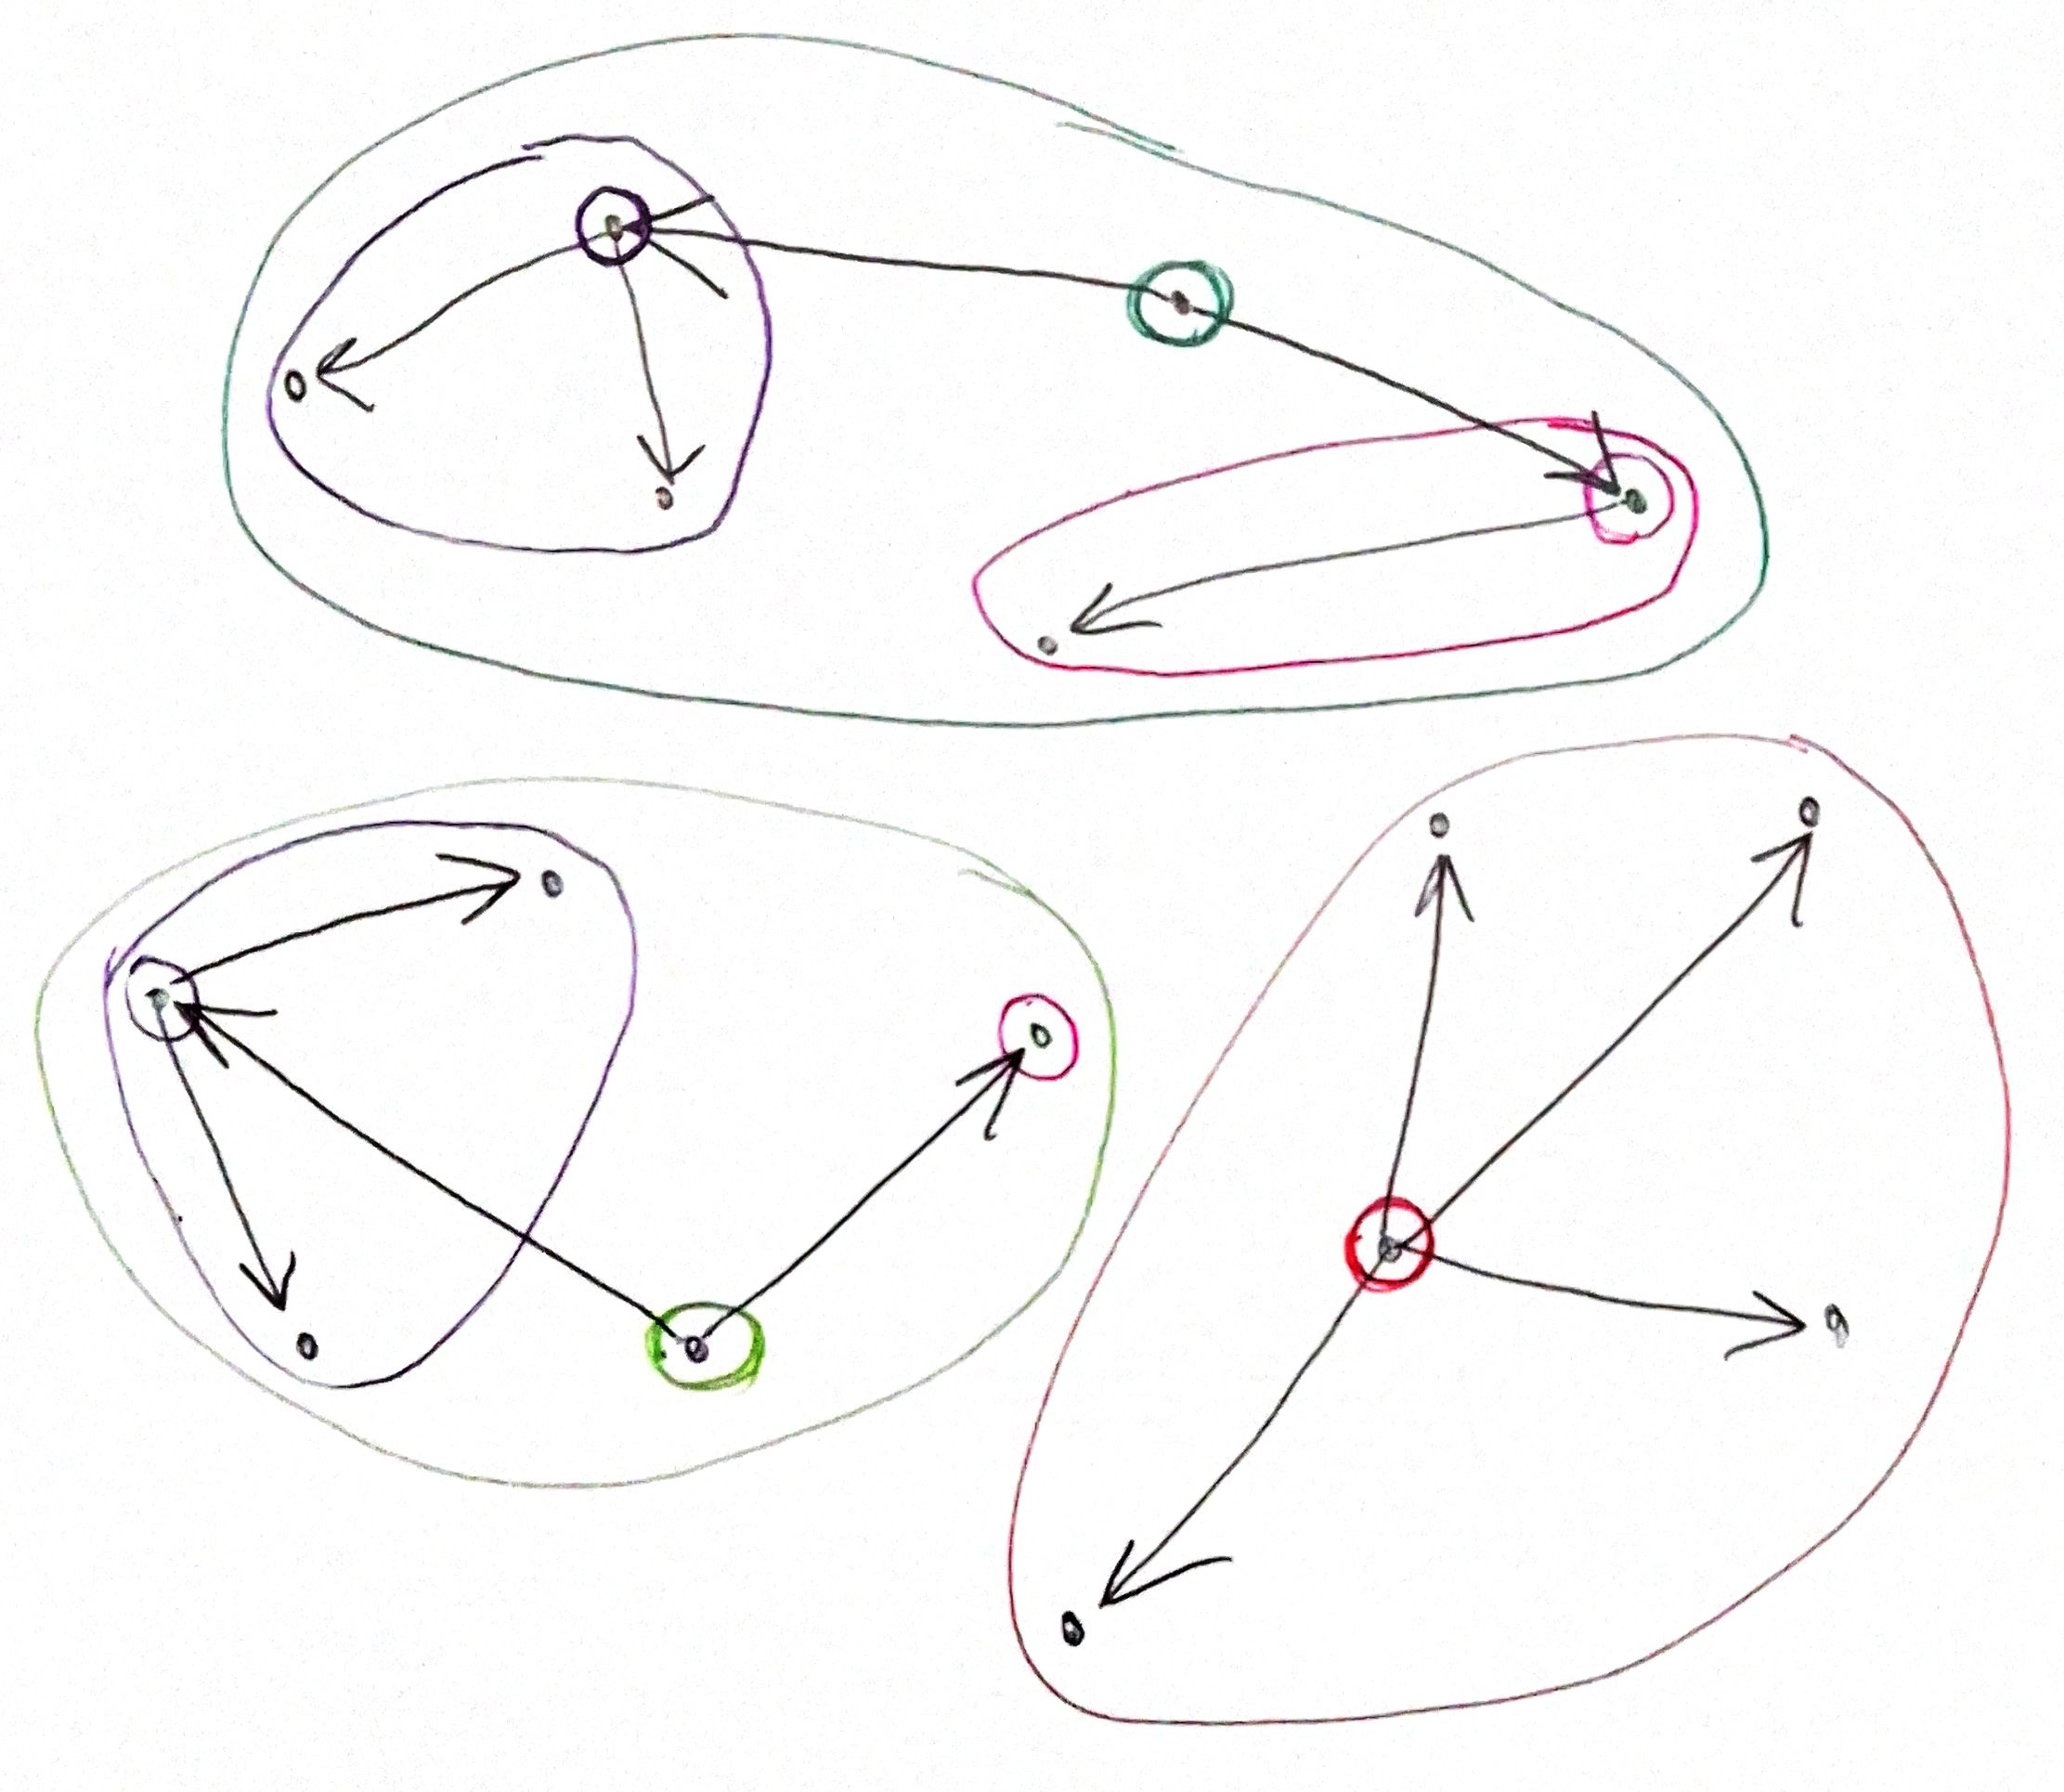
\includegraphics[width=0.5\textwidth]{images/precedence_construction.jpg}
    \caption{Precedence generation. The root nodes are the green, red and lemon. Red has four leaf vertices. Green has two branches, the pink with one leaf and the purple with two leaves. Lemon has one leaf and one branch with two leaves.}
    \label{fig:precedence-generation}
\end{figure}

\subsection{How to Generate the Weights}

Generate the weights randomly in the interval $\interval{0}{H}$.

\subsection{How to Generate the Knapsack Capacity}

Generate each entry of the knapsack capacity $\maximumWeight$ randomly in the interval $\interval{0}{m \cdot n \cdot H}$.

\subsection{\grasp}
\label{appendix:grasp}

\begin{algorithm}[H]
    \caption{\grasp}
    \label{algorithm:grasp}
    \begin{algorithmic}[1]
        \State{$S_{\mbox{best}} \gets \varnothing$}
        \For{$k = 1,\dots, N_{it}$}
            \State{$S \gets \mbox{Greedy-Randomized-Construction}()$}
            \State{$S \gets \mbox{Local-Search}(S$)}
            \State{$S_{\mbox{best}} \gets \max \Set{S, S_{\mbox{best}}}$}
        \EndFor
        \State{\textbf{return}\xspace $S_{\mbox{best}}$}
    \end{algorithmic}
\end{algorithm}

\begin{algorithm}[H]
    \caption{Greedy-Randomized-Construction($\alpha$)}
    \label{algorithm:grasp-construction}
    \begin{algorithmic}[1]
        \State{$S \gets \varnothing$}
        \State{$C \gets E$}
            \Comment{Candidates list}
        \For{$e \in C$}
            \State{$c(e) \gets \mbox{Incremental-Cost}(e, S)$}
                \Comment{Increment in the cost by adding $e$ to $S$}
        \EndFor
        \While{$C \neq \varnothing$}
            \State{$c_{min} = \min\Set{c(e) : e \in C}$}
            \State{$c_{max} = \max\Set{c(e) : e \in C}$}
            \State{$R \gets \Set{e \in C : c(e) \leqslant c_{min} + \alpha (c_{max} - c_{min})}$}
                \Comment{Restricted candidates list}
            \State{$s \gets \mbox{Select-Random-Element}(R)$}
            \State{$S \gets S \cup \Set{s}$}
            \State{Update $C$}
            \State{Update $c(e)$}
        \EndWhile
        \State{\textbf{return}\xspace $S$}
    \end{algorithmic}
\end{algorithm}

\begin{algorithm}[H]
    \caption{Loca-Search($S$)}
    \label{algorithm:grasp-local-search}
    \begin{algorithmic}[1]
        \While{$S$ is not local optimal}
            \State{$S \gets \argmax{S' \in N(S)}{f(S')}$}
                \Comment{$N(S)$ is the neighborhood of $S$}
                \Comment{$f$ is the goal function}
        \EndWhile
        \State{\textbf{return}\xspace $S$}
    \end{algorithmic}
\end{algorithm}

\subsection{\tabu}
\label{appendix:tabu}

\begin{algorithm}[H]
    \caption{\tabu($S_0$)}
    \label{algorithm:tabu}
    \begin{algorithmic}[1]
        \State{$S \gets S_0$}
            \Comment{$S_0$ is the initial solution}
            \Comment{$S$ is the current solution}
        \State{$S^* \gets S$}
            \Comment{$S^*$ is the current best solution}
        \State{$f^* \gets f(S^*)$}
            \Comment{$f$ is the goal function}
        \State{$T \gets \varnothing$}
            \Comment{$T$ is the tabu list}
        \While{not Termination-Criteria-Satisfied}
            \State{$S \gets \argmax{S' \in N(S, T)}{f(S')}$}
                \Comment{$N(S, T)$ is the neighborhood of $S$ limited by $T$}
            \If{$f(S) > f^*$}
                \State{$S^* \gets S$}
                \State{$f^* \gets f(S)$}
            \EndIf
            \State{Update $T$}
                \Comment{record moves and delete old entries}
        \EndWhile
        \State{\textbf{return}\xspace $S^*$}
    \end{algorithmic}
\end{algorithm}

\section{Implementação e execução dos experimentos}

O programs foram executados num ideapad S145 81S90005BR: Lenovo IdeaPad S145 Notebook Intel Core i5-8265U (6MB Cache, 1.6GHz, 8 cores), 8GB DDR4-SDRAM, 460 GB SSD, Intel UHD Graphics 620 no ambiente:

\begin{enumerate}
    \item sistema operacional: Fedora 35
    \item Java versão 17
    \item Gradle versão 7.4
\end{enumerate}

O desenvolvimento da solução do problema foi feito em Java, baseado nos frameworks disponibilizados pelos professores. O código pode ser encontrado em \cite{bib:github}.

\section{\tttfull (\ttt)}

\section{\perfprof}
\label{appendix:performance-profiles}

\begin{table}[H]
    \centering
        \begin{tabular}{|p{0.2\textwidth}||l|l|l|l|l|l|l|}

    \hline
    Problema & kqbf020 & kqbf040 & kqbf060 & kqbf080 & kqbf100 & kqbf200 & kqbf400 \\ \hline\hline
    \graspFirst & 0.145 & 0.353 & 1.261 & 3.016 & 6.056 & 75.552 & inf \\ \hline
    \graspBest & 0.074 & 1.765 & 1.981 & 4.242 & 9.068 & 100.731 & inf \\ \hline
    \tabuVanilla & 0.997 & 2.707 & 5.427 & 10.318 & 17.549 & 160.816 & inf \\ \hline
    \tabuMod & 0.255 & 1.218 & 5.662 & inf & 17.294 & 444.594 & inf \\ \hline
    \geneticVanilla & 0.974 & 3.200 & 5.529 & 9.627 & 15.386 & 62.351 & inf \\ \hline
    \geneticSteady & 3.015 & 10.860 & 23.954 & 46.665 & 76.459 & 254.404 & inf \\ \hline
    \end{tabular}
    \caption{Dados utilizados na confecção do \perfprof. \textit{inf} acima significa que o algoritmo não consegui resolver o problema, isto é, não encontrou uma solução com valor pelo menos o valor definido para o problema em questão.}
    \label{tab:data-perfprof}
\end{table}

\begin{figure}[H]
    \centering
    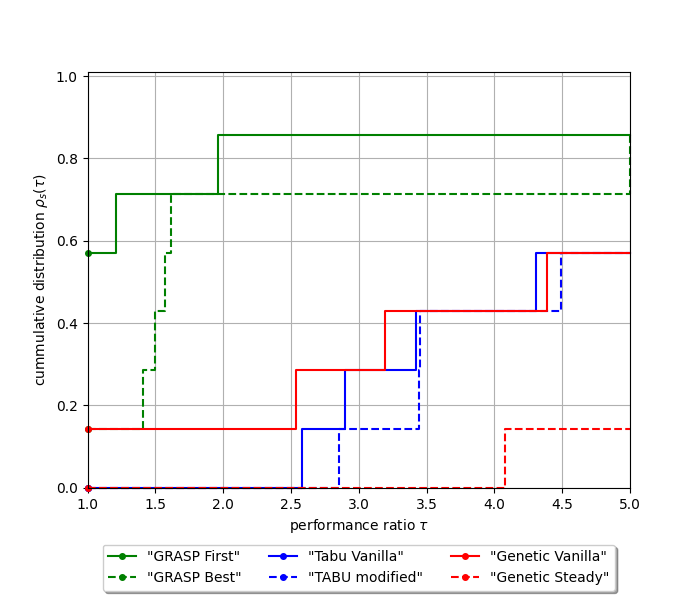
\includegraphics[width=\textwidth]{figure/performance_profile/performance_profile_thmax_5.0.png}
    \caption{Gráfico de \perfprof no intervalo $[1, 5]$}
    \label{fig:performance-profile-5}
\end{figure}

\begin{figure}[H]
    \centering
    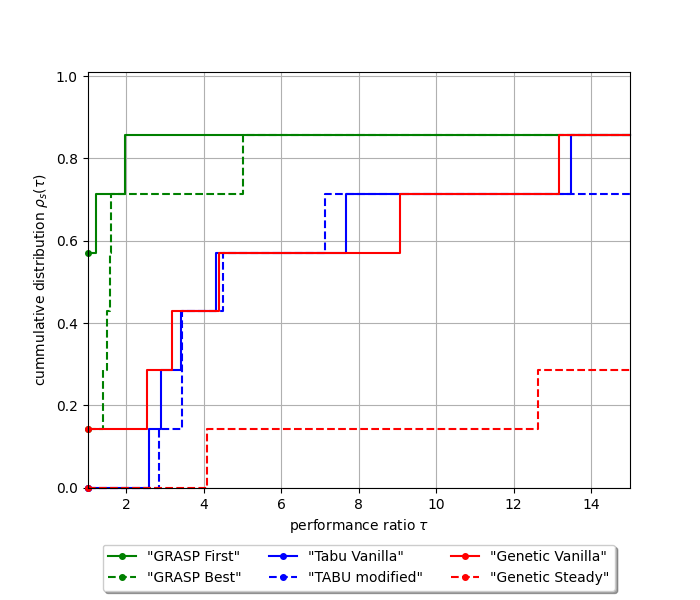
\includegraphics[width=\textwidth]{figure/performance_profile/performance_profile_thmax_15.0.png}
    \caption{Gráfico de \perfprof no intervalo $[1, 15]$}
    \label{fig:performance-profile-15}
\end{figure}

\begin{figure}[H]
    \centering
    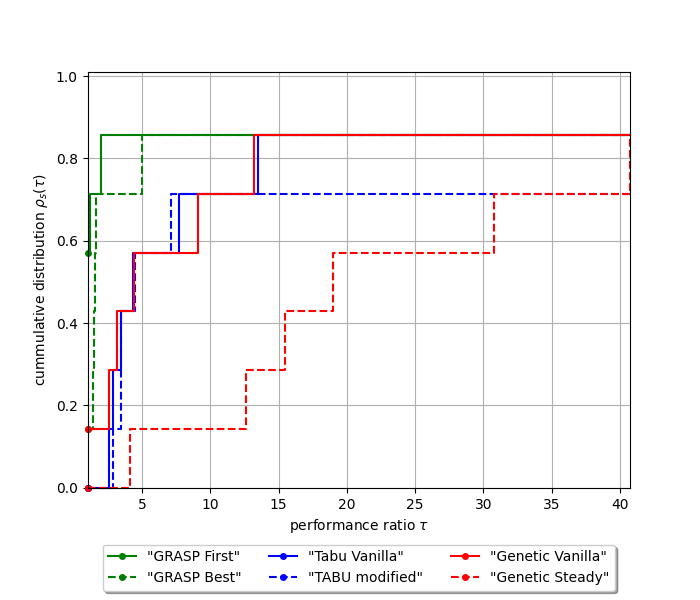
\includegraphics[width=\textwidth]{figure/performance_profile/performance_profile_thmax_None.png}
    \caption{Gráfico de \perfprof no intervalo $r_M$ (calculado automaticamente pelo software de plot).}
    \label{fig:performance-profile-max}
\end{figure}


\end{appendices}

\end{document}
